
\section{Modeling and Simulation}

\subsection{Modeling}

Causal.jl adopts causal modeling\footnote{Causal modeling is also known as signal flow modeling or block diagram modeling} approach in modeling systems. In causal modeling approach, a model consists of components and connections (Figure \ref{fig: simple model})\cite{matei2012modeling}. The simulation of the model is performed in a clocked environment. That is, the model is not simulated in one shot by solving a single mathematical equation system that represents the whole model, but instead, it is simulated by evolving the components between sampling intervals in parallel, individually.

The components interact with each other through the connections that are bound to their input/output ports. The components are data processing agents, and their behavior determines how the data is processed. Depending upon the nature of the system and the modeling, these equations may differ, i.e., they may or may not contain derivative terms, or they may contain the continuous or discrete-time variable, etc. The dataflow through the connections is unidirectional, i.e., a component is driven by other components that write data to its input port.

The model simulation is performed by evolving the components individually. A reference clock is used to make the components have a common time base. The clock generates pulses at simulation sampling intervals. These pulses are used to trigger the components during the run stage of the simulation. Each triggered component reads its input data from its input port, calculates its output according to its mathematical model, and writes the result to its output port.

\begin{figure}
    \centering
    \includegraphics[width=0.75\linewidth]{figures/Model/model.pdf}
    \caption{A model consisting of the components B1, $\ldots$, B5 and the connections L1, $\ldots$, L6. T is the common time reference of the model.}
    \label{fig: simple model}
\end{figure}


\subsection{Components}
The component types in Causal.jl are shown in Figure \ref{fig: component types}. The components can be classified as sources, sinks, and systems.

The sources are the components that generate outputs as functions of time only. When triggered, a source computes its output according to its readout function and writes the result to its output port. The sources do not have input ports.

The sinks are data processing units. Their primary goal is to process the data flowing through the connections online. When triggered, a sink reads its input data from its input port and processes it. The data can be visualized by being plotted on a graphical user interface, can be observed by being printed on a console, or can be recorded in data files. The sinks' data processing scope can be enriched by integrating new plugins that can be developed using the standard Julia library or various available Julia packages. Invariants, spectral properties, or statistical information can be extracted from the data. Parameter estimation can be performed, or various signal processing techniques can be applied. Causal.jl has been designed to be flexible enough to allow the users to extend its data analyzes scope by integrating newly-defined plugins.

\begin{figure}
    \centering
    \includegraphics[width=\linewidth]{figures/ComponentsCompressed/components_compresses.pdf}
    \caption{Component types in Causal.jl. $u, x, y$ signify the input, state, output of a system, respectively. $t$ and $k$ are continuous and discrete time variable, respectively. $W$ is the stochastic process corresponding to the noise and $x_\tau$ is the state $x$ delayed by $\tau$ seconds in time. $f$(and $h$) is the right-hand-side function of the differential equation representing the system and $g$ is the readout function.}
    \label{fig: component types}
\end{figure}

A static system is described by a readout equation solely. When triggered, a static system reads its input data from its input port, calculates its output according to its readout function, and writes the result to its output port. In dynamic systems, however, the system behavior is characterized by the states. The output of a dynamical system depends on its input, previous state(s), and time. Therefore, a dynamical system is described by a differential equation and a readout equation, classically. When triggered, a dynamical system reads its input from its input port, updates its state according to the differential equation, calculates its output according to its readout function, and writes the result to its output port. Being developed on top of DifferentialEquations.jl, Causal.jl is capable of simulating the dynamical systems represented by differential equations in the form of the ordinary differential equations(ODE), differential-algebraic equations(DAE), random ordinary differential equations(RODE), stochastic differential equations(SDE), delay differential equations(DDE) or discrete difference equations \cite{rackauckas2017differentialequations}. Most of the available simulation environments allow the systems represented by ordinary differential equations or differential-algebraic equations\cite{elmqvist1978structured,nytsch2006advanced,zimmer2008introducing,mosterman2002hybrsim,van2001variables,giorgidze2009higher,pfeiffer2012pysimulator,simulink}. Therefore, analyzes such as noise or delay analysis or unexpected change of system parameters cannot be performed in these simulation environments, easily. On the contrary, Causal.jl makes it possible for all these analyses to be performed owing to its ability to solve such a wide range of differential equations.

\subsection{Ports and Connections}
A port is a bunch of pins to which the connections are bound. There are two types of pins: an output pin that transfers data from the inside of the component to its outside, and an input pin that transfers data from the outside of the component to its inside. There are two types of ports: an output port that consists of output pins and an input port that consists of input pins.

\begin{figure}
    \centering
    \subfloat[]{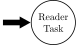
\includegraphics[width=0.225\linewidth]{figures/Tasks/reader_task.pdf} \label{subfig: reader task}} \hfil 
    \subfloat[]{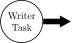
\includegraphics[width=0.225\linewidth]{figures/Tasks/writer_task.pdf} \label{subfig: writer task}} \hfil 
    \subfloat[]{\includegraphics[width=0.4\linewidth]{figures/Tasks/reader_writer_task.pdf} \label{subfig: reader writer task}} 
    \caption{\protect\subref{subfig: reader task} A readable connection, \protect\subref{subfig: writer task} A writable connection, \protect\subref{subfig: reader writer task} A readable and writable connection}
    \label{fig: tasks}
\end{figure}

The data transferred to a port are transferred to its connections. The data transfer through the connections is performed over the links of the connections. The links are built on top Julia channels. The data written to(read from) a link is written to(read from) its channel. Running Julia tasks bound to the channels must exist for the data to flow through these channels. Julia tasks are the control flow features that allow calculations to be flexibly suspended and maintained without directly communicating the task scheduler of the operating system\cite{julialang}. The communication and the data exchange between the tasks are carried out through Julia's channels to which they are bound.

Figure \ref{fig: tasks} depicts the tasks that must be bound to a connection to make it readable, writable, and both readable and writable, symbolically. The writer(the reader) task is the task that writes(reads) data to(from) the connection. A running writer task must be bound to the connection on the opposite side to read data from one side of a connection. This connection is called a readable connection. Similarly, to write data to one side of a connection, a running reader task must be bound to the connection at the other side. This connection is called a writable connection. If both running writer and reader tasks are bound to both sides of a connection, then the data can both be read from and written to the connection. Such a connection is called a readable and writable connection. The dataflow through a connection is only allowed if the connection is both readable and writable connection. The data read from a readable connection is the data written to the connection by the writer task of the connection. If the data have not been written to the connection by its writer task during a reading process yet, then reading does not occur, and the writer task is waited to put data to the connection. Similarly, if the data on a connection has not been read from the connection by its reader task during a writing process yet, then the reader task is waited to take data from the connection.

In the modeling approach adopted, the components reading data from a connection are driven by other components writing data to the connection. Therefore, all of the model's connections must be readable and writable so that data can flow through the connections. This necessitates that all the connections of the model must be connected to a component from both ends. Otherwise, the simulation gets stuck and does not terminate.

\subsection{Simulation}
A model to be simulated consists of components connected to each other and a time reference. The time reference is used to sample the continuous-time signals flowing through the model's connections and trigger the components. The simulation is performed by triggering the components with pulses generated by the time reference of the model at sampling time instants. When triggered, the components evolve to compute their outputs.

The simulation stages are shown in Figure \ref{fig: flowchart} basically. Performing, inspecting, and reporting all the simulation stages is carried out automatically without requiring any user intervention.

\begin{figure}
    \centering
    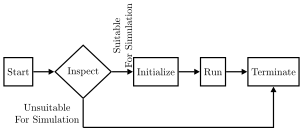
\includegraphics[width=\linewidth]{figures/FlowChart/flowchart.pdf}
    \caption{Flowchart of the simulation stages.}
    \label{fig: flowchart}
\end{figure}

\begin{figure}
    \centering
    \subfloat[]{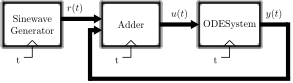
\includegraphics[width=0.49\linewidth]{figures/AlgebraicLoop/unbrokenloop.pdf} \label{subfig: unbroken algebraic loop}}
    \subfloat[]{\includegraphics[width=0.49\linewidth]{figures/AlgebraicLoop/brokenloop.pdf} \label{subfig: broken algebraic loop}}
    \caption{\protect\subref{subfig: unbroken algebraic loop} An algebraic loop consisting of the components Static System, Dynamical System I and Dynamical System II. \protect\subref{subfig: broken algebraic loop} Breaking of the loop with a Memory component. }
    \label{fig: algebraic loop}
\end{figure}

In the \textit{inspection} stage, the model is inspected to see whether the model is suitable for simulation. If connections having any unconnected terminals are detected, the simulation is terminated at this stage. The model is not suitable for simulation when algebraic loops exist\cite{lamego2001adaptive}. An algebraic loop is a closed-loop consisting of one or more components whose outputs are directly dependent on their inputs. Almost every system that includes feedbacks has algebraic loops. The simulation does not proceed because none of the components in the loop can generate output to break the loop. Such a problem can be solved by redesigning the model so that the model has no algebraic loops, solving the feed-forward algebraic equation of the loop, or inserting a memory component with a particular initial condition anywhere in the loop. Causal.jl provides all these loop-breaking solutions. During the \textit{inspection}, when algebraic loops are detected, all the loops are broken, if possible, automatically. Otherwise, a report is printed to notify the user to insert memory components to break the loops.

\begin{figure}
    \centering
    \subfloat[]{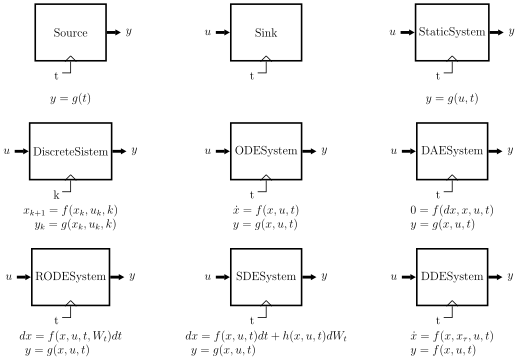
\includegraphics[width=0.5\linewidth]{figures/TaskForComponents/components.pdf} \label{subfig: components}} \\
    \subfloat[]{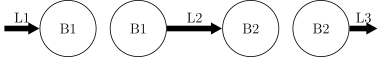
\includegraphics[width=.75\linewidth]{figures/TaskForComponents/tasks.pdf} \label{subfig: tasks}}
    \caption{Launching tasks for the connections. \protect\subref{subfig: components} An example model part consisting of the components B1 and B2 and the connections L1, L2 and L3. \protect\subref{subfig: tasks} Tasks launched corresponding to the connections.}
    \label{fig: tasks for components}
\end{figure}

If the model passes the \textit{inspection}, the writer and reader tasks are launched in the \textit{initialization} stage to ensure the data flow through the model connections. At this point, a writer and a reader task are bound to each connection. In Figure \ref{subfig: components} model part consisting of components B1, B2, and the connections L1, L2, L3 are shown. When triggered, the B1 reads data from L1, calculates its output, and writes to L2. Similarly, when triggered, B2 reads data from the L2, calculates its output, and writes to the L3. The tasks bounded to L1, L2, and L3 corresponding to B1 and B2 are shown in Figure \ref{subfig: tasks}. Since B1 reads the data from L1 and writes data to L2, a reader task is bounded to L1, and a writer task is bounded L2. Similarly, since B2 reads the data from L2 and writes data to L3, a reader task is bounded to L2, and a writer task is bounded L3. Since both a writer and a reader task are bound to the L2, data can flow from B1 to B2 through L2. A task manager is constructed to check whether the tasks launched during the \textit{initialization} are running correctly throughout the simulation.

The \textit{initialization} is followed by the \textit{run} stage. The tasks that are launched corresponding to the components during the \textit{initialization} expect the components to be triggered through their trigger pins. These triggers are generated in the sampling instants by the model clock during the \textit{run} stage. It is possible to sample the signals flowing through the connections at equal or independent time intervals. The generated triggers are put into the trigger pins of the components.

When the \textit{run} stage is completed, the tasks launched at the \textit{initialization} stage are closed in the \textit{termination} stage and the simulation ends.

The sampled values are interpolated for a duration of one sampling period so that the components can evolve independently. The sampling period is an essential factor that affects the accuracy of the simulation results directly.